\chapter{Material Models}
\label{cha:material:models}


\section{Specifying Material Properties}

Associating material properties with a given cell involves several
steps. 
\begin{enumerate}
\item In the mesh generation process, assign a material identifier to each
cell.
\item Define material property groups corresponding to each material identifier.
\item Set the parameters for each material group using \filename{.cfg} and/or command-line arguments.
\item Specify the spatial variation in material property parameters using
a spatial database file.
\end{enumerate}

\subsection{Setting the Material Identifier}

Each cell in the finite-element mesh must have a material identifier.
This integer value is associated with a bulk material model. The parameters
of the material model need not be uniform for cells with the same
material identifier. The bulk constitutive model and numerical integration
(quadrature) scheme will, however, be the same for all cells with
the same material identifier value. The material identifier is set
during the mesh generation process. The procedure for assigning this
integer value to a cell depends on the mesh generator. For example,
in the PyLith mesh ASCII format, the identifiers are listed in the
cells group using the material-id data; in CUBIT materials are defined
using blocks; in LaGriT materials are defined by the attribute \texttt{imt1}
and the mregion command.


\subsection{Material Property Groups}

The material property group associates a material model (label for the
material, a bulk constitutive model, and parameters for the
constitutive model) with a material identifier. In previous versions
of PyLith it was necessary to specify containers that defined the
number of groups and associated information for each group. This was
necessary because previous versions of Pyre did not support dynamic
arrays of components, and it was necessary to predefine these
arrays. More recent versions of Pythia do support this, however, and
it is now possible to define material property groups using a
\filename{.cfg} file or on the command-line. User-defined containers
are no longer necessary, and the predefined containers are no longer
available (or necessary). If a set of material groups is not
specified, a single material model is used for the entire problem. See
Sections \vref{sec:example:3dhex8} and \vref{sec:example:3dtet4}
for examples that demonstrate how to specify more than one material
model.


\subsection{Material Parameters}
\label{sec:material:parameters}

For each material group, there is a single component defining the
material model to be used. The default material model is \object{ElasticIsotropic3D}.
For each material model, the available properties and facilities are:
\begin{inventory}
\propertyitem{id}{This is the material identifier that matches the integer value
assigned to each cell in the mesh generation process.}
\propertyitem{label}{Name or label for the material. This is used in error and
diagnostic reports.}
\facilityitem{db\_properties}{Spatial database specifying the spatial variation
in the parameters of the bulk constitutive model (default is a SimpleDB).}
\facilityitem{db\_initial\_stress}{Spatial database specifying the spatial variation
in the initial stress (default is none).}
\facilityitem{db\_initial\_strain}{Spatial database specifying the spatial variation
in the initial strain (default is none).}
\facilityitem{db\_initial\_state}{Spatial database specifying the spatial variation
in the other initial state variables (default is none).}
\facilityitem{output}{The output manager used for outputting material information.}
\facilityitem{quadrature}{Numerical integration scheme used in integrating fields
over each cell.}
\end{inventory}
An example of setting these parameters in a \filename{.cfg} file for
a problem with two material groups is:
\begin{cfg}
<h>[pylithapp.timedependent]</h>
<p>materials</p> = [elastic,viscoelastic]

<h>[pylithapp.timedependent.materials.elastic]</h>
<p>label</p> = Elastic material
<p>id</p> = 1
<p>db_properties.iohandler.filename</p> = mat\_elastic.spatialdb
<f>quadrature.cell</f> = pylith.feassemble.FIATLagrange
<p>quadrature.cell.dimension</p> = 3

<h>[pylithapp.timedependent.materials.viscoelastic]</h>
<p>label</p> = Viscoelastic material
<p>id</p> = 2
<p>db_properties.iohandler.filename</p> = mat_viscoelastic.spatialdb
<f>quadrature.cell</f> = pylith.feassemble.FIATLagrange
<p>quadrature.cell.dimension</p> = 3
\end{cfg}

These settings correspond to the the problem in Section
\vref{sec:example:3dhex8}.  The parameters for the bulk constitutive
models are specified using the spatial databases
\filename{mat\_elastic.spatialdb} and
\filename{mat\_viscoelastic.spatialdb}.  Refer to the discussion of
each material model to find the parameters that must be specified in
the spatial database. Appendix \vref{sec:format:SimpleIOAscii}
describes the format of the SimpleDB spatial database files. In a more
realistic problem, a different spatial database, and possibly a
different material model, would be used for each material group.

In general, we average the output over the quadrature points within
a cell and specify the name of the output files for each material
group:
\begin{cfg}
<h>[pylithapp.timedependent.materials.elastic.output]</h>
<f>cell_filter</f> = pylith.meshio.CellFilterAvg
<p>writer.filename</p> = dislocation-elastic.vtk

<h>[pylithapp.timedependent.materials.viscoelastic.output]</h>
<f>cell_filter</f> = pylith.meshio.CellFilterAvg
<p>writer.filename</p> = dislocation-viscoelastic.vtk
\end{cfg}

These settings again correspond to the problem in Section \vref{sec:example:3dhex8}.
The specification of a state variable base filename (\filename{writer.filename}
settings) will cause two files to be created for each material group:
an info file, which describes the material property parameters used
in the model, and a state variables file, which contains the state
variable information. Note that the material property parameters described
by the info file are the parameters used internally by PyLith. In
some cases they are parameters convenient for use in the constitutive
models and are derived from the parameters specified by the user via
the spatial database. If the problem has more than one time step,
a state variable output file will be created for each requested time
step. We have requested that the values be averaged over each cell.
Otherwise, output would be produced for each quadrature point, which
can cause problems with some visualization packages. For this example
problem, the material is three-dimensional isotropic elastic, and
is thus described by three parameters ($\lambda$, $\mu$, $\rho$),
as described below. These properties are output by default. Other
material models require additional parameters, and if users want these
to be output, they must be specified. Similarly, other material models
require state variables in addition to the default stress and strain
variables that are used by all material models. Additional output
may be requested for a material model, as in this example (see Section
\vref{sec:example:twohex8}):
\begin{cfg}
<h>[pylithapp.timedependent.materials.material.output]</h>
<p>cell_data_fields</p> = [total_strain, viscous_strain, stress]
<p>cell_info_fields</p> = [mu, lambda, density, maxwell_time]
\end{cfg}

The properties and state variables available for output in each
material model are listed in Table
\vref{tab:materials:output}. The order of the state variables in
the output arrays is given in Table \vref{tab:materials:statevars}.
For the generalized Maxwell model, values of \texttt{shear\_ratio} and
\texttt{maxwell\_time} are given for each Maxwell element in the model
(there are presently three, as described below). Similarly, there are
three sets of \texttt{viscous\_strain} values for the generalized
Maxwell model.

\begin{table}[htbp]
\caption{Properties and state variables available for output for
  existing material models. Physical properties are available for
  output as \property{cell\_info\_fields} and state variables are
  available for output as \property{cell\_data\_fields}.}
\label{tab:materials:output}

\begin{tabular}{p{1.5in}p{1.8in}p{1.5in}p{1in}}
\textbf{Model} & \textbf{Physical Properties} & \textbf{State Variables} & \textbf{Requires nonlinear solver?}\tabularnewline
\hline 
Elastic & \texttt{mu, lambda, density} & \texttt{total\_strain, stress, cauchy\_stress} & No\\
Maxwell Viscoelastic & \texttt{mu, lambda, density, maxwell\_time} & \texttt{total\_strain,} \texttt{stress, cauchy\_stress, viscous\_strain} & No\\
Generalized Maxwell Viscoelastic & \texttt{mu, lambda, density,} \texttt{shear\_ratio,} \texttt{maxwell\_time} & \texttt{total\_strain, stress, cauchy\_stress, viscous\_strain\_1,} \texttt{viscous\_strain\_2,} \texttt{viscous\_strain\_3} & No\\
Power-law Viscoelastic & \texttt{mu, lambda, density,} \texttt{reference\_strain\_rate, reference\_stress,} 
\texttt{power\_law\_exponent} & \texttt{total\_strain, stress, cauchy\_stress, viscous\_strain} & Yes\\
Drucker-Prager Elastoplastic & \texttt{mu, lambda, density, alpha\_yield},\texttt{ beta, alpha\_flow } & \texttt{total\_strain, stress, cauchy\_stress, plastic\_strain} & Yes\\
\hline 
\end{tabular}
\end{table}

\begin{table}[htbp]
\caption{Order of components in tensor state-variables for material models.}
\label{tab:materials:statevars}
\begin{tabular}{p{2.5in}p{1.5in}p{2.0in}}
\textbf{State Variable} & \textbf{2D} & \textbf{3D}\\
\hline 
\texttt{total\_strain} & $\epsilon_{xx}$, $\epsilon_{yy}$, $\epsilon_{xy}$ & $\epsilon_{xx}$, $\epsilon_{yy}$, $\epsilon_{zz}$, $\epsilon_{xy}$,
$\epsilon_{yz}$, $\epsilon_{xz}$\\
\texttt{stress, cauchy\_stress} & $\sigma_{xx}$, $\sigma_{yy}$, $\sigma_{xy}$ & $\sigma_{xx}$, $\sigma_{yy}$, $\sigma_{zz}$, $\sigma_{xy}$, $\sigma_{yz}$,
$\sigma_{xz}$\\
\texttt{viscous\_strain, plastic\_strain} & $\epsilon_{xx}$, $\epsilon_{yy}$, $\epsilon_{zz}$, $\epsilon_{xy}$ & $\epsilon_{xx}$, $\epsilon_{yy}$, $\epsilon_{zz}$, $\epsilon_{xy}$,
$\epsilon_{yz}$, $\epsilon_{xz}$\\
\texttt{stress4} & $\sigma_{xx}$, $\sigma_{yy}$, $\sigma_{zz}$, $\sigma_{xy}$ & \\
\hline 
\end{tabular}
\end{table}


\subsection{Initial State Variables}
\label{sec:materials:reference:state}

In many problems of interest, the state variables describing a material
model may already have nonzero values prior to the application of
any boundary conditions. For problems in geophysics, the most common
example is a problem that includes the effects of gravitational body
forces. In the real earth, rocks were emplaced and formed under the
influence of gravity. When performing numerical simulations, however,
it is not possible to represent the entire time history of rock emplacement.
Instead, gravity must be ``turned on'' at the beginning of the simulation.
Unfortunately, this results in unrealistic amounts of deformation
at the beginning of a simulation. An alternative is to provide initial
state variables for the region under consideration. This allows the
specification of a set of state variables that is consistent with
the prior application of gravitational body forces. In a more general
sense, initial values for state variables may be used to provide values
that are consistent with any set of conditions that occurred prior
to the beginning of a simulation. The current release of PyLith allows
the specification of initial stresses, strains, and state variables
for all materials; however, not all of the initial state variables
are presently used. For example, \texttt{cauchy\_stress} is available
as a state variable for all materials, but specifying an initial value
would not make sense for most problems.


\subsubsection{Specification of Initial State Variables}

State variables are specific to a given material, so initial values
for state variables are specified as part of the material description.
The default is that no initial state variables are specified. In computing
the elastic prestep, appropriate values for the state variables are
set; otherwise the state variables are set to zero. To override this
behavior, specify a spatial database for the initial stress, strain,
and/or state variables as in the example from the example in Section
\vref{sec:example:3dhex8}:
\begin{cfg}
<h>[pylithapp.timedependent.materials.elastic]</h>
<f>db_initial_stress</f> = spatialdata.spatialdb.SimpleDB
<p>db_initial_stress.iohandler.filename<p> = initial\_stress.spatialdb
\end{cfg}

\warning{Using the elastic prestep with initial state variables will
  generally lead to the state variables being ignored (the initial out
  of plane stress is the exception), because the elastic prestep will
  set the state variables based on the elastic solution.}

\warning{Currently, PyLith assumes initial displacements and
  velocities of zero, so any initial strain and state variables should
  be consistent with these initial conditions.  This limitation will
  be removed in future releases.}

As mentioned in section \vref{sec:materials:formulations:viscoelastic}, plane
strain problems do not include the out-of-plane stress component ($\sigma_{zz}$),
and an additional state variable (\texttt{stress-zz-initial}) is provided
for all two-dimensional viscoelastic and elastoplastic models. To
completely specify the initial stresses, the user must provide two
spatial databases: an initial stress database that includes the three
2D stress components ($\sigma_{xx}$, $\sigma_{yy}$, and $\sigma_{xy}$)
and an additional database containing the out of plane stress and
initial values for all other state variables for the given material.
The complete initial stress field may then be defined in the \filename{.cfg}
file as:
\begin{cfg}
<h>[pylithapp.problem.materials.powerlaw]</h>
# First specify initial 2D stresses
<f>db_initial_stress</f> = spatialdata.spatialdb.SimpleDB
<p>db_initial_stress.label</p> = 2D initial stress
<p>db_initial_stress.iohandler.filename</p> = inititial_stress_2d.spatialdb

# Now specify out-of-plane initial stresses (and all other state variables)
<f>db_initial_state</f> = spatialdata.spatialdb.SimpleDB
<p>db_initial_state.label</p> = Out of plane strain initial stress
<p>db_initial_state.iohandler.filename</p> = initial_state_2d.spatialdb
\end{cfg}

\begin{table}[htbp]
\caption{Values in spatial database for initial state variables for 3D
  problems.  2D problems use only the relevant values. Note that
  initial stress and strain are available for all material
  models. Some models have additional state variables (Table
  \vref{tab:materials:output}) and initial values for these may
  also be provided.}
\begin{tabular}{p{0.85in}p{5.0in}}
\textbf{State Variable} & \textbf{Values in Spatial Database}\\
\hline 
initial stress & \texttt{stress-xx, stress-yy, stress-zz, stress-xy, stress-yz, stress-xz}\\
initial strain & \texttt{total-strain-xx, total-strain-yy, total-strain-zz, total-strain-xy,
total-strain-yz, total-strain-xz}\\
\hline 
\end{tabular}
\end{table}


\subsection{Cauchy Stress Tensor and Second Piola-Kirchoff Stress Tensor}

In outputting the stress tensor (see Tables
\vref{tab:materials:output} and \vref{tab:materials:statevars}),
the tensor used internally in the formulation of the governing
equation is the \texttt{stress} field available for output. For the
infinitesimal strain formulation this is the Cauchy stress tensor; for
the finite strain formulation, this is the second Piola-Kirchoff
stress tensor. The user may also explicitly request output of the
Cauchy stress tensor (\texttt{cauchy\_stress} field). Obviously, this
is identical to the \texttt{stress} field when using the infinitesimal
strain formulation.  See section \vref{sec:small:strain:formulation}
for a discussion of the relationship between the Cauchy stress tensor
and the second Piola-Kirchhoff stress tensor.

\important{Although the second Piola-Kirchoff stress tensor has little
  physical meaning, the second Piola-Kirchoff stress tensor (not the
  Cauchy stress tensor) values should be specified in the initial
  stress database when using the finite strain formulation.}

\subsection{Stable time step}
\label{sec:stable:time:step}

PyLith computes the stable time step in both quasi-static and dynamic
simulations. In quasi-static simulations the stability of the implicit
time stepping scheme does not depend on the time step; instead, the
stable time step is associated with the accuracy of the solution.  For
viscoelastic materials the stable time step uses 1/5 of the minimum
viscoelastic relaxation time. In purely elastic materials, the
accuracy is independent of the time step, so the stable time step is
infinite.  The same is true for elastoplastic materials, since there
is no inherent time scale for these problems. Depending on the loading
rate, however, it is possible to impose a load increment that is large
enough so that the resulting solution may be inaccurate or divergent.
In quasi-static simulations we recompute the stable time step at every
time step.

\warning{Caution must be used in assigning time step sizes for
  elastoplastic problems, and the linear and nonlinear convergence
  should be monitored closely.}

In dynamic simulations the stability of the explicit time-stepping
scheme integration does depend on the time step via the Courant-Friderichs-Lewy
condition \cite{Courant:etal:1967}. This condition states that the
critical time step is the time it takes for the P wave to travel across
the shortest dimension of a cell. In most cases this is the shortest
edge length. However, distorted cells which have relatively small
areas in 2-D or relatively small volumes in 3-D for the given edge
lengths also require small time steps due to the artificially high
stiffness associated with the distorted shape. As a result, we set
the stable time step to be the smaller of the shortest edge length
and a scaling factor times the radius of an inscribed circle (in 2-D),
\begin{gather}
dt=\min(e_{\mathit{min}},3.0r_{inscribed})\\
r_{inscribed}=\sqrt{\frac{k(k-e_{0})(k-e_{1})(k-e_{2})}{k}}\\
k=\frac{1}{2}(e_{0}+e_{1}+e_{2})
\end{gather}
and sphere (in 3-D),
\begin{gather}
dt=\min(e_{\mathit{min}},6.38r_{inscribed})\\
r_{inscribed}=3V/(A_{0}+A_{1}+A_{2}+A_{3}),
\end{gather}
where $e_{i}$ denotes the length of edge $i$, $A_{i}$ denotes the
area of face $i$, and $V$ is the volume of the cell. We determined
the scaling factoring empirically using several benchmarks. In dynamic
simulations we check the stable time step only at the beginning of
the simulation. That is, we assume the elastic properties and mesh
do not change, so that the stable time step is constant throughout
the simulation.

The stable time step is used in all three of the time stepping schemes
used by PyLith (see section \vref{sec:time-stepping}). In general,
an error is generated if the user attempts to use a time step size
larger than the stable time step. The stable time steps for each cell
can be included in the output with the other \property{cell\_info\_fields}.
For implicit time stepping the field is \texttt{stable\_dt\_implicit}
and for explicit time stepping the field is \texttt{stable\_dt\_explicit}.


\section{Elastic Material Models}

The generalized form of Hooke's law relating stress and strain for
linear elastic materials is

\begin{gather}
\sigma_{ij}=C_{ijkl}\left(\epsilon_{kl}-\epsilon_{kl}^{I}\right)+\sigma_{ij}^{I}\,,\label{eq:1}
\end{gather}
where we have included both initial strains and initial stresses,
denoted with the superscript \textsl{I}. Due to symmetry considerations,
however, the 81 components of the elasticity matrix are reduced to
21 independent components for the most general case of anisotropic
elasticity. Representing the stress and strain in terms of vectors,
the constitutive relation may be written
\begin{gather}
\overrightarrow{\sigma}=\underline{C}\left(\vec{\epsilon}-\vec{\epsilon}^{I}\right)+\vec{\sigma}^{I},\label{eq:2}
\end{gather}
where

\begin{gather}
\underline{C}=\left[\begin{array}{cccccc}
C_{1111} & C_{1122} & C_{1133} & C_{1112} & C_{1123} & C_{1113}\\
C_{1122} & C_{2222} & C_{2233} & C_{2212} & C_{2223} & C_{2213}\\
C_{1133} & C_{2233} & C_{3333} & C_{3312} & C_{3323} & C_{3313}\\
C_{1112} & C_{2212} & C_{3312} & C_{1212} & C_{1223} & C_{1213}\\
C_{1123} & C_{2223} & C_{3323} & C_{1223} & C_{2323} & C_{2313}\\
C_{1113} & C_{2213} & C_{3313} & C_{1213} & C_{2313} & C_{1313}
\end{array}\right]\:.\label{eq:3}
\end{gather}
For the case of isotropic elasticity, the number of independent components
reduces to two, and the model can be characterized by two parameters,
Lame's constants $\mu$ and $\lambda$. Lame's constants are related
to the density ($\rho$), shear wave speed ($v_{s}$), and compressional
wave speed ($v_{p}$) via
\begin{equation}
\begin{aligned}\mu= & \rho v_{s}^{2}\\
\lambda= & \rho v_{p}^{2}-2\mu
\end{aligned}
\label{eq:4}
\end{equation}

\begin{table}[htbp]
  \caption{Values in spatial databases for the elastic material
    constitutive models.}
\begin{tabular}{lll}
\textbf{Spatial database} & \textbf{Value} & \textbf{Description}\\
\hline 
\facility{db\_properties} & \texttt{vp} & Compressional wave speed, $v_{p}$\\
 & \texttt{vs} & Shear wave speed, $v_{s}$\\
 & \texttt{density} & Density, $\rho$\\
\facility{db\_initial\_stress} & \texttt{stress-xx}, \ldots & Initial stress components\\
\facility{db\_initial\_strain} & \texttt{total-strain-xx}, \ldots & Initial strain components\\
\hline 
\end{tabular}
\end{table}


\subsection{2D Elastic Material Models}

In 2D we can write Hooke's law as
\begin{gather}
\left[\begin{array}{c}
\sigma_{11}\\
\sigma_{22}\\
\sigma_{12}
\end{array}\right]=\left[\begin{array}{ccc}
C_{1111} & C_{1122} & C_{1112}\\
C_{1122} & C_{2222} & C_{2212}\\
C_{1112} & C_{2212} & C_{1212}
\end{array}\right]\left[\begin{array}{c}
\epsilon_{11}-\epsilon_{11}^{I}\\
\epsilon_{22}-\epsilon_{22}^{I}\\
\epsilon_{12}-\epsilon_{12}^{I}
\end{array}\right]+\left[\begin{array}{c}
\sigma_{11}^{I}\\
\sigma_{22}^{I}\\
\sigma_{12}^{I}
\end{array}\right]\:.\label{eq:9}
\end{gather}


\subsubsection{Elastic Plane Strain}

If the gradient in deformation with respect to the $x_{3}$ axis is
zero, then $\epsilon_{33}=\epsilon_{13}=\epsilon_{23}=0$ and plane
strain conditions apply, so we have 
\begin{gather}
\left[\begin{array}{c}
\sigma_{11}\\
\sigma_{22}\\
\sigma_{12}
\end{array}\right]=\left[\begin{array}{ccc}
\lambda+2\mu & \lambda & 0\\
\lambda & \lambda+2\mu & 0\\
0 & 0 & 2\mu
\end{array}\right]\left[\begin{array}{c}
\epsilon_{11}-\epsilon_{11}^{I}\\
\epsilon_{22}-\epsilon_{22}^{I}\\
\epsilon_{12}-\epsilon_{12}^{I}
\end{array}\right]+\left[\begin{array}{c}
\sigma_{11}^{I}\\
\sigma_{22}^{I}\\
\sigma_{12}^{I}
\end{array}\right]\:.\label{eq:10}
\end{gather}


\subsubsection{Elastic Plane Stress}

If the $x_{1}x_{2}$ plane is traction free, then $\sigma_{33}=\sigma_{13}=\sigma_{23}=0$
and plane stress conditions apply, so we have
\begin{gather}
\left[\begin{array}{c}
\sigma_{11}\\
\sigma_{22}\\
\sigma_{12}
\end{array}\right]=\left[\begin{array}{ccc}
\frac{4\mu(\lambda+\mu)}{\lambda+2\mu} & \frac{2\mu\lambda}{\lambda+2\mu} & 0\\
\frac{2\mu\lambda}{\lambda+2} & \frac{4\mu(\lambda+\mu)}{\lambda+2\mu} & 0\\
0 & 0 & 2\mu
\end{array}\right]\left[\begin{array}{c}
\epsilon_{11}-\epsilon_{11}^{I}\\
\epsilon_{22}-\epsilon_{22}^{I}\\
\epsilon_{12}-\epsilon_{12}^{I}
\end{array}\right]+\left[\begin{array}{c}
\sigma_{11}^{I}\\
\sigma_{22}^{I}\\
\sigma_{12}^{I}
\end{array}\right]\:,\label{eq:11}
\end{gather}
where
\begin{equation}
\begin{gathered}\epsilon_{33}=-\frac{\lambda}{\lambda+2\mu}(\epsilon_{11}+\epsilon_{22})+\epsilon_{33}^{I}\\
\epsilon_{13}=\epsilon_{23}=0\,.
\end{gathered}
\label{eq:12}
\end{equation}

\subsection{3D Elastic Material Models}

\subsubsection{Isotropic}

For this case the stress-strain matrix, $\underline{C}$, becomes
\begin{gather}
\underline{C}=\left[\begin{array}{cccccc}
\lambda+2\mu & \lambda & \lambda & 0 & 0 & 0\\
\lambda & \lambda+2\mu & \lambda & 0 & 0 & 0\\
\lambda & \lambda & \lambda+2\mu & 0 & 0 & 0\\
0 & 0 & 0 & 2\mu & 0 & 0\\
0 & 0 & 0 & 0 & 2\mu & 0\\
0 & 0 & 0 & 0 & 0 & 2\mu
\end{array}\right]\:.\label{eq:13}
\end{gather}


\section{Viscoelastic Materials}
\label{sec:materials:viscoelastic}

At present, there are six viscoelastic material models available in
PyLith (Table \vref{tab:materials:viscoelastic} and Figure
\vref{fig:material:models}). Future code versions may include alternative
formulations for the various material models (Appendix \vref{cha:materials:alternative:formulations}),
so that users may use the most efficient formulation for a particular
problem. Note that both 2D and 3D viscoelastic models are described,
but we present below only the 3D formulations. The 2D formulations
are easily obtained from the plane strain definition. The one aspect
of the 2D formulations that is different is the specification of initial
stresses. Since 2D models only have three tensor components, it is
not possible to specify the normal stress in the out-of-plane direction
($\sigma_{33}$), which is generally nonzero, using the same method
as the other tensor components. To allow for the specification of
this initial stress component, an additional state variable corresponding
to $\sigma_{33}^{I}$ is provided (\texttt{stress\_zz\_initial}).
This state variable is provided for all of the viscoelastic material
models as well as the plane strain Drucker-Prager elastoplastic model.
See section \vref{sec:materials:reference:state} for additional information
on specifying initial stresses for plane strain problems. For the
PowerLawPlaneStrain model, all four of the stress components are needed,
so a 4-component stress state variable (\texttt{stress4}) is provided
in addition to the normal 3-component \texttt{stress} state variable
(see Table \vref{tab:materials:output}).

\begin{table}[htbp]
\caption{Available viscoelastic materials
for PyLith.}
\label{tab:materials:viscoelastic}
\begin{tabular}{p{1.5in}p{4.5in}}
\textbf{Model Name} & \textbf{Description}\\
\hline 
\object{MaxwellPlaneStrain} & Plane strain Maxwell material with linear viscous rheology\\
\object{GenMaxwellPlaneStrain} & Plane strain generalized Maxwell material (3 Maxwell models in parallel)\\
\object{PowerLawPlaneStrain} & Plane strain Maxwell material with power-law viscous rheology\\
\object{MaxwellIsotropic3D} & Isotropic Maxwell material with linear viscous rheology\\
\object{GenMaxwellIsotropic3D} & Generalized model consisting of 3 Maxwell models in parallel\\
\object{PowerLaw3D} & Isotropic Maxwell material with power-law viscous rheology\\
\hline 
\end{tabular}
\end{table}

\begin{figure}[htbp]
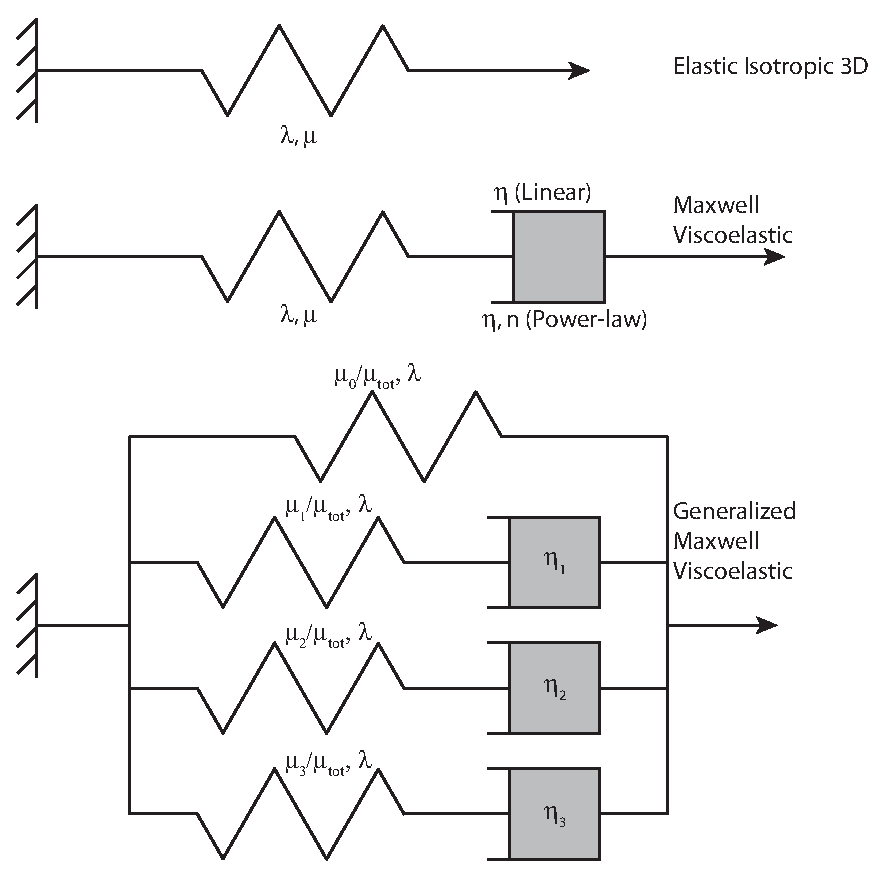
\includegraphics[scale=0.75]{materials/figs/pylith-materials}
\caption{Spring-dashpot 1D representations of the available 3D elastic
  and 2D/3D viscoelastic material models for PyLith.  The top model is
  a linear elastic model, the middle model is a Maxwell model, and the
  bottom model is a generalized Maxwell model. For the generalized
  Maxwell model, $\lambda$ and $\mu_{tot}$ are specified for the
  entire model, and then the ratio $\mu_{i}/\mu_{tot}$ is specified
  for each Maxwell model. For the power-law model, the linear dashpot
  in the Maxwell model is replaced by a nonlinear dashpot obeying a
  power-law.}
\label{fig:material:models}
\end{figure}


\subsection{Definitions}

In the following sections, we use a combination of vector and index
notation (our notation conventions are shown in Table \vref{tab:notation}).
When using index notation, we use the common convention where repeated
indices indicate summation over the range of the index. We also make
frequent use of the scalar inner product. The scalar inner product
of two second-order tensors may be written
\begin{gather}
\underline{a}\cdot\underline{b}=a_{ij}b_{ij}\,.\label{eq:14}
\end{gather}
Although the general constitutive relations are formulated in terms
of the stress and strain, we frequently make use of the deviatoric
stress and strain in our formulation. We first define the mean stress,
$P$, and mean strain, $\theta$:
\begin{gather}
P=\frac{\sigma_{ii}}{3}\,,\,\,\,\,\theta=\frac{\epsilon_{ii}}{3}\,,\label{eq:15}
\end{gather}
where the $\sigma_{ii}$ and $\epsilon_{ii}$ represent the trace
of the stress and strain tensors, respectively. We then define the
deviatoric components of stress and strain as
\begin{gather}
S_{ij}=\sigma_{ij}-P\delta_{ij}\,,\,\,\,\, e_{ij}=\epsilon_{ij}-\theta\delta_{ij}\,,\label{eq:16}
\end{gather}
where $\delta_{ij}$ is the Kronecker delta. Using the deviatoric
components, we define the effective stress, $\overline{\sigma}$,
the second deviatoric stress invariant, $J_{2}^{\prime}$, the effective
deviatoric strain, $\overline{e}$, and the second deviatoric strain
invariant, $L_{2}^{\prime}$, as
\begin{gather}
\overline{\sigma}=\sqrt{\frac{3}{2}\underline{S}\cdot\underline{S}}\,\,\nonumber \\
J_{2}^{\prime}=\frac{1}{2}\underline{S}\cdot\underline{S}\,.\label{eq:17}\\
\overline{e}=\sqrt{\frac{2}{3}\underline{e}\cdot\underline{e}}\,\,\nonumber \\
L_{2}^{\prime}=\frac{1}{2}\underline{e}\cdot\underline{e}\,\,\nonumber 
\end{gather}
Due to the symmetry of the stress and strain tensors, it is sometimes
convenient to represent them as vectors:
\begin{gather}
\overrightarrow{\sigma^{T}}=\left[\begin{array}{cccccc}
\sigma_{11} & \sigma_{22} & \sigma_{33} & \sigma_{12} & \sigma_{23} & \sigma_{31}\end{array}\right]\label{eq:18}\\
\overrightarrow{\epsilon^{T}}=\left[\begin{array}{cccccc}
\epsilon_{11} & \epsilon_{22} & \epsilon_{33} & \epsilon_{12} & \epsilon_{23} & \epsilon_{31}\end{array}\right]\:.\nonumber 
\end{gather}
Note that when taking the scalar inner product of two tensors represented
as vectors, it is necessary to double the products representing off-diagonal
terms.

For quantities evaluated over a specific time period, we represent
the initial time as a prefixed subscript and the end time as a prefixed
superscript. In cases where the initial time does not appear, it is
understood to be $-\infty$.

\subsection{Linear Viscoelastic Models}

Linear viscoelastic models are obtained by various combinations of
a linear elastic spring and a linear viscous dashpot in series or
parallel. The simplest example is probably the linear Maxwell model,
which consists of a spring in series with a dashpot, as shown in Figure
\vref{fig:material:models}. For a one-dimensional model, the response
is given by
\begin{equation}
\frac{d\epsilon_{Total}}{dt}=\frac{d\epsilon_{D}}{dt}+\frac{d\epsilon_{S}}{dt}=\frac{\sigma}{\eta}+\frac{1}{E}\frac{d\sigma}{dt}\:,
\end{equation}
where $\epsilon_{Total}$ is the total strain, $\epsilon_{D}$ is
the strain in the dashpot, $\epsilon_{S}$ is the strain in the spring,
$\sigma$ is the stress, $\eta$ is the viscosity of the dashpot,
and $E$ is the spring constant. When a Maxwell material is subjected
to constant strain, the stresses relax exponentially with time. When
a Maxwell material is subjected to a constant stress, there is an
immediate elastic strain, corresponding to the response of the spring,
and a viscous strain that increases linearly with time. Since the
strain response is unbounded, the Maxwell model actually represents
a fluid.

Another simple model is the Kelvin-Voigt model, which consists of
a spring in parallel with a dashpot. In this case, the one-dimensional
response is given by
\begin{equation}
\sigma\left(t\right)=E\epsilon\left(t\right)+\eta\frac{d\epsilon\left(t\right)}{dt}\:.
\end{equation}
As opposed to the Maxwell model, which represents a fluid, the Kelvin-Voigt
model represents a solid undergoing reversible, viscoelastic strain.
If the material is subjected to a constant stress, it deforms at a
decreasing rate, gradually approaching the strain that would occur
for a purely elastic material. When the stress is released, the material
gradually relaxes back to its undeformed state.

The most general form of linear viscoelastic model is the generalized
Maxwell model, which consists of a spring in parallel with a number
of Maxwell models (see Figure \vref{fig:material:models}). Using this
model, it is possible to represent a number of simpler viscoelastic
models. For example, a simple Maxwell model is obtained by setting
the elastic constants of all springs to zero, with the exception of
the spring contained in the first Maxwell model ($\mu_{1}$). Similarly,
the Kelvin-Voigt model may be obtained by setting the elastic constants
$\mu_{2}=\mu_{3}=0$, and setting $\mu_{1}=\infty$ (or a very large
number).


\subsection{Formulation for Generalized Maxwell Models}
\label{sec:materials:formulation:generalized:Maxwell}

As described above, the generalized Maxwell viscoelastic model consists
of a number of Maxwell linear viscoelastic models in parallel with
a spring, as shown in Figure \vref{fig:material:models}. PyLith includes
the specific case of a spring in parallel with three Maxwell models.
As described in the previous paragraph, a number of common material
models may be obtained from this model by setting the shear moduli
of various springs to zero or infinity (or a large number), such as
the Maxwell model, the Kelvin model, and the standard linear solid.
We follow formulations similar to those used by Zienkiewicz and Taylor
\cite{Zienkiewicz:Taylor:2000} and Taylor \cite{Taylor:2003}. In
this formulation, we specify the total shear modulus of the model
($\mu_{tot}$) and Lame's constant ($\lambda$). We then provide the
fractional shear modulus for each Maxwell element spring in the model.
It is not necessary to specify the fractional modulus for $\mu_{0}$,
since this is obtained by subtracting the sum of the other ratios
from 1. Note that the sum of all these fractions must equal 1. We
use a similar formulation for our linear Maxwell viscoelastic model,
but in that case $\mu_{0}$ is always zero and we only use a single
Maxwell model. The parameters defining the standard Maxwell model
are shown in Table \vref{tab:materials:linear:Maxwell}, and those defining the
generalized Maxwell model are shown in Table \vref{tab:materials:generalized:Maxwell}.

As for all our viscoelastic models, the volumetric strain is completely
elastic, and the viscoelastic deformation may be expressed purely
in terms of the deviatoric components:
\begin{equation}
\underline{S}=2\mu_{tot}\left[\mu_{0}\underline{e}+\sum_{i=1}^{N}\mu_{i}\underline{q}^{i}-\underline{e}^{I}\right]+\underline{S}^{I}\,;\; P=3K\left(\theta-\theta^{I}\right)+P^{I}\,,\label{eq:19}
\end{equation}
where \textsl{K} is the bulk modulus, $N$ is the number of Maxwell
models, and the variable $\underline{q}^{i}$ follows the evolution
equations
\begin{equation}
\underline{\dot{q}}^{i}+\frac{1}{\tau_{i}}\underline{q}^{i}=\underline{\dot{e}}.\label{eq:20}
\end{equation}
The $\tau_{i}$ are the relaxation times for each Maxwell model:
\begin{equation}
\tau_{i}=\frac{\eta_{i}}{\mu_{tot}\mu_{i}}\:.\label{eq:21-1}
\end{equation}

An alternative to the differential equation form above is an integral
equation form expressed in terms of the relaxation modulus function.
This function is defined in terms of an idealized experiment in which,
at time labeled zero ($t=0$), a specimen is subjected to a constant
strain, $\underline{e}_{0}$, and the stress response, $\underline{S}\left(t\right)$,
is measured. For a linear material we obtain:
\begin{equation}
\underline{S}\left(t\right)=2\mu\left(t\right)\left(\underline{e}_{0}-\underline{e}^{I}\right)+\underline{S}^{I}\,,\label{eq:21}
\end{equation}
where $\mu\left(t\right)$ is the shear relaxation modulus function.
Using linearity and superposition for an arbitrary state of strain
yields an integral equation:
\begin{equation}
\underline{S}\left(t\right)=\intop_{-\infty}^{t}\mu\left(t-T\right)\underline{\dot{e}}\, dT\,.\label{eq:22}
\end{equation}
If we assume the modulus function in Prony series form we obtain
\begin{equation}
\mu\left(t\right)=\mu_{tot}\left(\mu_{0}+\sum_{i=1}^{N}\mu_{i}\exp\frac{-t}{\tau_{i}}\right)\,,\label{eq:23}
\end{equation}
where
\begin{equation}
\mu_{0}+\sum_{i=1}^{N}\mu_{i}=1\,.\label{eq:24}
\end{equation}
With the form in Equation \vref{eq:23}, the integral equation form
is identical to the differential equation form.

If we assume the material is undisturbed until a strain is suddenly
applied at time zero, we can divide the integral into
\begin{equation}
\intop_{-\infty}^{t}\left(\cdot\right)\, dT=\intop_{-\infty}^{0^{-}}\left(\cdot\right)\, dT+\intop_{0^{-}}^{0^{+}}\left(\cdot\right)\, dT+\intop_{0^{+}}^{t}\left(\cdot\right)\, dT\,.\label{eq:27}
\end{equation}
The first term is zero, the second term includes a jump term associated
with $\underline{e}_{0}$ at time zero, and the last term covers the
subsequent history of strain. Applying this separation to Equation
\vref{eq:22},
\begin{equation}
\underline{S}\left(t\right)=2\mu\left(t\right)\left(\underline{e}_{0}-\underline{e}^{I}\right)+\underline{S}^{I}+2\int_{0}^{t}\mu\left(t-T\right)\underline{\dot{e}}\left(T\right)\, dT\,,\label{eq:28}
\end{equation}
where we have left the sign off of the lower limit on the integral.

Substituting Equation \vref{eq:23} into \vref{eq:28}, we obtain
\begin{equation}
\underline{S}\left(t\right)=2\mu_{tot}\left\{ \mu_{0}\underline{e}\left(t\right)+\sum_{i=1}^{N}\left[\mu_{i}\exp\frac{-t}{\tau_{i}}\left(\underline{e}_{0}+\intop_{0}^{t}\exp\frac{t}{\tau_{i}}\underline{\dot{e}}\left(T\right)\, dT\right)\right]-\underline{e}^{I}\right\} +\underline{S}^{I}\,.\label{eq:29}
\end{equation}
We then split each integral into two ranges: from 0 to $t_{n}$, and
from $t_{n}$ to $t$, and define each integral as
\begin{equation}
\underline{i}_{i}^{1}\left(t\right)=\intop_{0}^{t}\exp\frac{T}{\tau_{i}}\underline{\dot{e}}\left(T\right)\, dT\,.\label{eq:30}
\end{equation}
The integral then becomes
\begin{equation}
\underline{i}_{i}^{1}\left(t\right)=\underline{i}_{i}^{1}\left(t_{n}\right)+\intop_{t_{n}}^{t}\exp\frac{T}{\tau_{i}}\underline{\dot{e}}\left(T\right)\, dT\,.\label{eq:31}
\end{equation}
Including the negative exponential multiplier:
\begin{equation}
\underline{h}_{i}^{1}\left(t\right)=\exp\frac{-t}{\tau_{i}}\underline{i}_{i}^{1}\,.\label{eq:32}
\end{equation}
Then
\begin{equation}
\underline{h}_{i}^{1}\left(t\right)=\exp\frac{-\Delta t}{\tau_{i}}\underline{h}_{i}^{1}\left(t_{n}\right)+\Delta\underline{h}_{i}\,,\label{eq:33}
\end{equation}
where
\begin{equation}
\Delta\underline{h}_{i}=\exp\frac{-t}{\tau_{i}}\intop_{t_{n}}^{t}\exp\frac{T}{\tau_{i}}\underline{\dot{e}}\left(T\right)\, dT\,.\label{eq:34}
\end{equation}
Approximating the strain rate as constant over each time step, the
solution may be found as
\begin{equation}
\Delta\underline{h}_{i}=\frac{\tau_{i}}{\Delta t}\left(1-\exp\frac{-\Delta t}{\tau_{i}}\right)\left(\underline{e}-\underline{e}_{n}\right)=\Delta h_{i}\left(\underline{e}-\underline{e}_{n}\right)\,.\label{eq:35}
\end{equation}
The approximation is singular for zero time steps, but a series expansion
may be used for small time-step sizes:
\begin{equation}
\Delta h_{i}\approx1-\frac{1}{2}\left(\frac{\Delta t}{\tau_{i}}\right)+\frac{1}{3!}\left(\frac{\Delta t}{\tau_{i}}\right)^{2}-\frac{1}{4!}\left(\frac{\Delta t}{\tau_{i}}\right)^{3}+\cdots\,.\label{eq:36}
\end{equation}
This converges with only a few terms. With this formulation, the constitutive
relation now has the simple form:
\begin{equation}
\underline{S}\left(t\right)=2\mu_{tot}\left(\mu_{0}\underline{e}\left(t\right)+\sum_{i=1}^{N}\mu_{i}\underline{h}_{i}^{1}\left(t\right)-\underline{e}^{I}\right)+\underline{S}^{I}\,.\label{eq:37}
\end{equation}


We need to compute the tangent constitutive matrix when forming the
stiffness matrix. In addition to the volumetric contribution to the
tangent constitutive matrix, we require the deviatoric part:
\begin{equation}
\frac{\partial\underline{S}}{\partial\underline{\epsilon}}=\frac{\partial\underline{S}}{\partial\underline{e}}\frac{\partial\underline{e}}{\partial\underline{\epsilon}}\,,\label{eq:38}
\end{equation}
where the second derivative on the right may be easily deduced from
Equation \vref{eq:16}. The other derivative is given by
\begin{equation}
\frac{\partial\underline{S}}{\partial\underline{e}}=2\mu_{tot}\left[\mu_{0}\underline{I}+\sum_{i=1}^{N}\mu_{i}\frac{\partial\underline{h}_{i}^{1}}{\partial\underline{e}}\right]\,,\label{eq:39}
\end{equation}
where $\underline{I}$ is the identity matrix. From Equations \vref{eq:33}
through \vref{eq:35}, the derivative inside the brackets is
\begin{equation}
\frac{\partial\underline{h}_{i}^{1}}{\partial\underline{e}}=\Delta h_{i}\left(\Delta t\right)\underline{I}\,.\label{eq:40}
\end{equation}
The complete deviatoric tangent relation is then
\begin{equation}
\frac{\partial\underline{S}}{\partial\underline{\epsilon}}=2\mu_{tot}\left[\mu_{0}+\sum_{i=1}^{N}\mu_{i}\Delta h_{i}\left(\Delta t\right)\right]\frac{\partial\underline{e}}{\partial\underline{\epsilon}}\,.\label{eq:41}
\end{equation}


We use this formulation for both our Maxwell and generalized Maxwell
viscoelastic models. For the Maxwell model, $\mu_{0}=0$ and $N=1$.
For the generalized Maxwell model, $N=3.$ The stable time step is
equal to 1/5 of the minimum relaxation time for all of the Maxwell
models (equation \vref{eq:21-1}).

\begin{table}[htbp]
\caption{Values in spatial databases for the linear Maxwell viscoelastic material constitutive model.}
\label{tab:materials:linear:Maxwell}
\begin{tabular}{lll}
\textbf{Spatial database} & \textbf{Value} & \textbf{Description}\\
\hline 
\facility{db\_properties} & \texttt{vp} & Compressional wave speed, $v_{p}$\\
 & \texttt{vs} & Shear wave speed, $v_{s}$\\
 & \texttt{density} & Density, $\rho$\\
 & \texttt{viscosity} & Viscosity, $\eta$\\
\facility{db\_initial\_stress} & \texttt{stress-xx}, \ldots & Initial stress components\\
\facility{db\_initial\_strain} & \texttt{total-strain-xx}, \ldots & Initial strain components\\
\facility{db\_initial\_state} & \texttt{viscous-strain-xx}, \ldots & Initial viscous strain components\\
 & \texttt{stress-zz-initial} & Initial out-of-plane stress (2D only)\\
\hline 
\end{tabular}
\end{table}

\begin{table}[htbp]
\caption{Values in spatial database used as parameters in the
  generalized linear Maxwell viscoelastic material constitutive
  model.}
\label{tab:materials:generalized:Maxwell}
\begin{tabular}{lll}
\textbf{Spatial database} & \textbf{Value} & \textbf{Description}\\
\hline 
\facility{db\_properties} & \texttt{vp} & Compressional wave speed, $v_{p}$\\
 & \texttt{vs} & Shear wave speed, $v_{s}$\\
 & \texttt{density} & Density, $\rho$\\
 & \texttt{shear-ratio-1} & Shear ratio for Maxwell model 1, $\mu_{1}/\mu_{tot}$\\
 & \texttt{shear-ratio-2} & Shear ratio for Maxwell model 2, $\mu_{2}/\mu_{tot}$\\
 & \texttt{shear-ratio-3} & Shear ratio for Maxwell model 3, $\mu_{3}/\mu_{tot}$\\
 & \texttt{viscosity-1} & Viscosity for Maxwell model 1, $\eta_{1}$\\
 & \texttt{viscosity-2} & Viscosity for Maxwell model 2, $\eta_{2}$\\
 & \texttt{viscosity-3} & Viscosity for Maxwell model 3, $\eta_{3}$\\
\facility{db\_initial\_stress} & \texttt{stress-xx}, \ldots & Initial stress components\\
\facility{db\_initial\_strain} & \texttt{total-strain-xx}, \ldots & Initial strain components\\
\facility{db\_initial\_state} & \texttt{viscous-strain-1-xx}, \ldots & Initial viscous strain components for Maxwell model 1\\
 & \texttt{viscous-strain-2-xx}, \ldots & Initial viscous strain components for Maxwell model 2\\
 & \texttt{viscous-strain-3-xx}, \ldots & Initial viscous strain components for Maxwell model 3\\
 & \texttt{stress-zz-initial} & Initial out-of-plane stress (2D only)\\
\hline 
\end{tabular}
\end{table}


\subsection{Effective Stress Formulations for Viscoelastic Materials}
\label{sec:materials:formulation:viscoelastic:effective}

As an alternative to the approach outlined above, an effective stress
function formulation \cite{Kojic:Bathe:1987} may be employed for
both a linear Maxwell model and a power-law Maxwell model. Note that
this formulation is not presently employed for linear viscoelastic
models (see Appendix \vref{cha:materials:alternative:formulations}), but it
is used for power-law viscoelastic materials. For the viscoelastic
materials considered here, the viscous volumetric strains are zero
(incompressible flow), and it is convenient to separate the general
stress-strain relationship at time $t+\Delta t$ into deviatoric and
volumetric parts:
\begin{gather}
\phantom{}{}^{t+\Delta t}\underline{S}=\frac{E}{1+\nu}\left(^{t+\Delta t}\underline{e}-\phantom{}^{t+\Delta t}\underline{e}^{C}-\underline{e}^{I}\right)+\underline{S}^{I}=\frac{1}{a_{E}}\left(^{t+\Delta t}\underline{e}-\phantom{}^{t+\Delta t}\underline{e}^{C}-\underline{e}^{I}\right)\label{eq:42}\\
^{t+\Delta t}P=\frac{E}{1-2\nu}\left(^{t+\Delta t}\theta-\theta^{I}\right)+P^{I}=\frac{1}{a_{m}}\left(^{t+\Delta t}\theta-\theta^{I}\right)\:,\nonumber 
\end{gather}
where $^{t+\Delta t}\underline{e}$ is the total deviatoric strain,
$^{t+\Delta t}\underline{e}^{C}$ is the total viscous strain, $\underline{e}^{I}$
is the initial deviatoric strain, $^{t+\Delta t}P$ is the pressure,
$^{t+\Delta t}\theta$ is the mean strain evaluated at time $t+\Delta t$
, and $\theta^{I}$ is the initial mean strain. The initial deviatoric
stress and initial pressure are given by $\underline{S}^{I}$ and
$P^{I}$, respectively. The topmost equation in Equation \vref{eq:42}
may also be written as
\begin{gather}
^{t+\Delta t}\underline{S}=\frac{1}{a_{E}}(^{t+\Delta t}\underline{e}^{\prime}-\underline{\Delta e}^{C})+\underline{S}^{I}\,,\label{eq:43}
\end{gather}
where
\begin{gather}
^{t+\Delta t}\underline{e}^{\prime}=\phantom{}^{t+\Delta t}\underline{e}-\phantom{}^{t}\underline{e}^{C}-\underline{e}^{I}\,\,,\,\,\,\underline{\Delta e}^{C}=\phantom{}^{t+\Delta t}\underline{e}^{C}-\phantom{}^{t}\underline{e}^{C}\,.\label{eq:44}
\end{gather}
The creep strain increment is approximated using
\begin{gather}
\underline{\Delta e}^{C}=\Delta t\phantom{}^{\tau}\gamma\phantom{}^{\tau}\underline{S}\,,\label{eq:45}
\end{gather}
where, using the $\alpha$-method of time integration,
\begin{gather}
^{\tau}\underline{S}=(1-\alpha)_{I}^{t}\underline{S}+\alpha\phantom{}_{I}^{t+\Delta t}\underline{S}+\underline{S}^{I}=(1-\alpha)^{t}\underline{S}+\alpha\phantom{}^{t+\Delta t}\underline{S}\,\,,\label{eq:46}
\end{gather}
and
\begin{gather}
^{\tau}\gamma=\frac{3\Delta\overline{e}^{C}}{2\Delta t\phantom{}^{\tau}\overline{\sigma}}\,\,,\label{eq:47}
\end{gather}
where
\begin{gather}
\Delta\overline{e}^{C}=\sqrt{\frac{2}{3}\underline{\Delta e}^{C}\cdot\underline{\Delta e}^{C}}\label{eq:48}
\end{gather}
and
\begin{gather}
^{\tau}\overline{\sigma}=(1-\alpha)_{I}^{t}\overline{\sigma}+\alpha\phantom{}_{I}^{t+\Delta t}\overline{\sigma}+\overline{\sigma}^{I}=\sqrt{3\phantom{}^{\tau}J_{2}^{\prime}}\,\,.\label{eq:49}
\end{gather}


To form the global stiffness matrix, it is necessary to provide a
relationship for the viscoelastic tangent material matrix relating
stress and strain. If we use vectors composed of the stresses and
tensor strains, this relationship is
\begin{gather}
\underline{C}^{VE}=\frac{\partial\phantom{}^{t+\Delta t}\overrightarrow{\sigma}}{\partial\phantom{}^{t+\Delta t}\overrightarrow{\epsilon}}\,\,.\label{eq:55}
\end{gather}
In terms of the vectors, we have
\begin{gather}
^{t+\Delta t}\sigma_{i}=\phantom{}^{t+\Delta t}S_{i}+\phantom{}^{t+\Delta t}P\,\,;\,\,\, i=1,2,3\label{eq:56}\\
^{t+\Delta t}\sigma_{i}=\phantom{}^{t+\Delta t}S_{i}\,;\,\,\,\,\,\,\,\,\,\,\,\,\,\,\,\,\,\,\,\,\,\,\,\,\,\,\,\,\,\,\, i=4,5,6\nonumber 
\end{gather}
Therefore,
\begin{gather}
C_{ij}^{VE}=C_{ij}^{\prime}+\frac{1}{3a_{m}}\,;\,\,1\leq i,j\leq3\,\,.\label{eq:57}\\
C_{ij}^{VE}=C_{ij}^{\prime}\,;\,\,\,\,\,\,\,\,\,\,\,\,\,\,\,\,\,\,\,\,\,\,\,\,\,\,\,\,\,\,\,\,\,\,\,\textrm{otherwise}\nonumber 
\end{gather}
Using the chain rule,
\begin{gather}
C_{ij}^{\prime}=\frac{\partial\phantom{}^{t+\Delta t}S_{i}}{\partial\phantom{}^{t+\Delta t}\epsilon_{j}}=\frac{\partial\phantom{}^{t+\Delta t}S_{i}}{\partial\phantom{}^{t+\Delta t}e_{k}^{\prime}}\frac{\partial\phantom{}^{t+\Delta t}e_{k}^{\prime}}{\partial\phantom{}^{t+\Delta t}e_{l}}\frac{\partial\phantom{}^{t+\Delta t}e_{l}}{\partial\phantom{}^{t+\Delta t}\epsilon_{j}}\,\,.\label{eq:58}
\end{gather}
From Equation \vref{eq:44}, we obtain
\begin{gather}
\frac{\partial\phantom{}^{t+\Delta t}e_{k}^{\prime}}{\partial\phantom{}^{t+\Delta t}e_{l}}=\delta_{kl}\,\,,\label{eq:59}
\end{gather}
and from Equation \vref{eq:16}:
\begin{gather}
\frac{\partial\phantom{}^{t+\Delta t}e_{l}}{\partial\phantom{}^{t+\Delta t}\epsilon_{j}}=\frac{1}{3}\left[\begin{array}{ccc}
2 & -1 & -1\\
-1 & 2 & -1\\
-1 & -1 & 2
\end{array}\right];\,\,1\leq l,j\leq3\label{eq:60}\\
\frac{\partial\phantom{}^{t+\Delta t}e_{l}}{\partial\phantom{}^{t+\Delta t}\epsilon_{j}}=\delta_{lj}\,\,;\,\,\,\,\,\,\,\,\,\,\,\,\,\,\,\,\,\,\,\,\,\,\,\,\,\,\,\,\,\,\,\,\,\,\,\,\,\,\,\,\,\,\,\,\textrm{otherwise.}\nonumber 
\end{gather}
The first term of Equation \vref{eq:58} depends on the particular
constitutive relationship, and the complete tangent matrix may then
be obtained from Equation \vref{eq:57}.


\subsubsection{Power-Law Maxwell Viscoelastic Material}
\label{sec:materials:formulation:powerlaw}

Laboratory results on rock rheology are typically performed using
a triaxial experiment, and the creep data are fit to a power-law equation
of the form (e.g., \cite{Kirby:Kronenberg:1987}):
\begin{equation}
\dot{\epsilon}_{11}^{C}=A_{E}\exp\left(\frac{-Q}{RT}\right)\left(\sigma_{1}-\sigma_{3}\right)^{n}=A_{E}\exp\left(\frac{-Q}{RT}\right)\sigma_{d}^{n}\:,\label{eq:64}
\end{equation}
where $\dot{\epsilon}_{11}^{C}$ is the strain rate in the direction
of the maximum principal stress $\left(\sigma_{1}\right)$, $A_{E}$
is the experimentally-derived pre-exponential constant, $Q$ is the
activation enthalpy, $R$ is the universal gas constant, $T$ is the
absolute temperature, $n$ is the power-law exponent, $\sigma_{3}\:\left(=\sigma_{2}\right)$
is equal to the confining pressure, and $\sigma_{d}$ is the differential
stress. To properly formulate the flow law, it must be generalized
so that the results are not influenced by the experiment type or the
choice of coordinate systems (e.g., \cite{Paterson:1994}). The flow
law may then be generalized in terms of the deviatoric stress and
strain rate invariants:
\begin{equation}
\sqrt{\dot{L}_{2}^{\prime C}}=A_{M}\exp\left(\frac{-Q}{RT}\right)\sqrt{J_{2}^{\prime}}^{n}\:,\label{eq:65}
\end{equation}
where $A_{M}$ is now a pre-exponential constant used in the formulation
for modeling. In practice, it is necessary to compute each strain
rate component using the flow law. This is accomplished using:
\begin{equation}
\dot{e}_{ij}^{C}=A_{M}\exp\left(\frac{-Q}{RT}\right)\sqrt{J_{2}^{\prime}}^{n-1}S_{ij}\:.\label{eq:66}
\end{equation}
Note that Equations \vref{eq:65} and \vref{eq:66} are consistent,
since Equation \vref{eq:65} may be obtained from Equation \vref{eq:66}
by taking the scalar inner product of both sides, multiplying by 1/2,
and taking the square root.

In a triaxial experiment with confining pressure $P_{c}$, we have
\begin{gather}
\sigma_{2}=\sigma_{3}=P_{c}\nonumber \\
\sigma_{1}=\sigma_{1}^{app}\label{eq:67}\\
P=\frac{\sigma_{1}+2P_{c}}{3}\:,\nonumber 
\end{gather}
where $\sigma_{1}^{app}$ is the applied load. The deviatoric stresses
are then:
\begin{gather}
S_{1}=\frac{2}{3}\left(\sigma_{1}-P_{c}\right)\nonumber \\
S_{2}=S_{3}=-\frac{1}{3}\left(\sigma_{1}-P_{c}\right)\:.\label{eq:68}
\end{gather}
This gives
\begin{gather}
S_{1}=\frac{2}{3}\left(\sigma_{1}-\sigma_{3}\right)=\frac{2}{3}\sigma_{d}\nonumber \\
S_{2}=S_{3}=-\frac{1}{3}\left(\sigma_{1}-\sigma_{3}\right)=-\frac{1}{3}\sigma_{d}\:.\label{eq:69}
\end{gather}
In terms of the second deviatoric stress invariant, we then have
\begin{equation}
\sqrt{J_{2}^{\prime}}=\frac{\sigma_{d}}{\sqrt{3}}\:.\label{eq:70}
\end{equation}

Under the assumption that the creep measured in the laboratory experiments
is incompressible, we have
\begin{gather}
\dot{e}_{11}^{C}=\dot{\epsilon}_{11}\nonumber \\
\dot{e}_{22}^{C}=\dot{e}_{33}^{C}=-\frac{1}{2}\dot{\epsilon}_{11}\:.\label{eq:71}
\end{gather}
In terms of the second deviatoric strain rate invariant we then have
\begin{equation}
\sqrt{\dot{L}_{2}^{\prime C}}=\frac{\sqrt{3}}{2}\dot{\epsilon}_{11}\:.\label{eq:72}
\end{equation}
Substituting Equations \vref{eq:70} and \vref{eq:72} into Equation
\vref{eq:64}, we obtain
\begin{equation}
\sqrt{\dot{L}_{2}^{\prime C}}=A_{E}\frac{\sqrt{3}^{n+1}}{2}\exp\left(\frac{-Q}{RT}\right)\sqrt{J_{2}^{\prime}}^{n}\:,\label{eq:73}
\end{equation}
and therefore,
\begin{equation}
A_{M}=\frac{\sqrt{3}^{n+1}}{2}A_{E}\:.\label{eq:74}
\end{equation}
When the exponential factor is included, we define a new parameter:
\begin{equation}
A_{T}=A_{M}\exp\left(\frac{-Q}{RT}\right)=\frac{\sqrt{3}^{n+1}}{2}A_{E}\exp\left(\frac{-Q}{RT}\right)\:.\label{eq:75}
\end{equation}

There is a problem with the usage of parameters $A_{E}$, $A_{M}$,
and $A_{T}$. Since the dimensions of these parameters are dependent
on the value of the power-law exponent, they are not really constants.
In addition to being logically inconsistent, this presents problems
when specifying parameters for PyLith, since the power-law exponent
must be known before the units can be determined. An alternative way
of writing the flow rule is (e.g., \cite{Prentice:1968}): 
\begin{equation}
\frac{\sqrt{\dot{L}_{2}^{\prime C}}}{\dot{e}_{0}}=\left(\frac{\sqrt{J_{2}^{\prime}}}{S_{0}}\right)^{n},\label{eq:76}
\end{equation}
where $\dot{e}_{0}$ and $S_{0}$ are reference values for the strain
rate and deviatoric stress. This means that
\begin{equation}
\frac{\dot{e}_{0}}{S_{0}^{n}}=A_{T}\:.\label{eq:77}
\end{equation}
Users must therefore specify three parameters for a power-law material.
The properties \texttt{reference-strain-rate}, \texttt{reference-stress},
and \texttt{power-law-exponent} in Table \vref{tab:materials:powerlaw} refer
to $\dot{e}_{0}$, $S_{0}$, and $n$, respectively. To specify the
power-law properties for PyLith using laboratory results, the user
must first compute $A_{T}$ using Equation \vref{eq:75}. Then, values
for $\dot{e}_{0}$ and $S_{0}$ must be provided. The simplest method
is probably to assume a reasonable value for the reference strain
rate, and then compute $S_{0}$ as
\begin{equation}
S_{0}=\left(\frac{\dot{e}_{0}}{A_{T}}\right)^{\frac{1}{n}}\:.\label{eq:78}
\end{equation}

A utility code (\texttt{powerlaw\_gendb.py}) is provided to convert
laboratory results to the properties used by PyLith. To use the code,
users must specify the spatial variation of $A_{E}$, $Q$, $n$,
and $T$. An additional parameter is given to define the units of
$A_{E}$. The user then specifies either a reference stress or a reference
strain rate, and a database suitable for PyLith is generated. This
utility is described more fully in Section \vref{sec:example:3dhex8:step08}.

The flow law in component form is 
\begin{equation}
\dot{e}_{ij}^{C}=\frac{\dot{e}_{0}\sqrt{J_{2}^{\prime}}^{n-1}S_{ij}}{S_{0}^{n}}\:,\label{eq:79}
\end{equation}
and the creep strain increment is approximated as
\begin{gather}
\underline{\Delta e}^{C}\approx\frac{\Delta t\dot{e}_{0}\sqrt{^{\tau}J_{2}^{\prime}}^{n-1}\,^{\tau}\underline{S}}{S_{0}^{n}}=\frac{\Delta t\dot{e}_{0}\phantom{}^{\tau}\overline{\sigma}^{n-1}\,^{\tau}\underline{S}}{\sqrt{3}S_{0}^{n}}\,.\label{eq:80}
\end{gather}
 Therefore,
\begin{gather}
\Delta\bar{e}^{C}\approx\frac{2\Delta t\dot{e}_{0}\sqrt{^{\tau}J_{2}^{\prime}}^{n}}{\sqrt{3}S_{0}^{n}}=\frac{2\Delta t\dot{e}_{0}\phantom{}^{\tau}\overline{\sigma}^{n}}{\sqrt{3}^{n+1}S_{0}^{n}}\,,\,\textrm{and}\,^{\tau}\gamma=\frac{\dot{e}_{0}\sqrt{^{\tau}J_{2}^{\prime}}^{n-1}}{S_{0}^{n}}\,.\label{eq:81}
\end{gather}
substituting Equations \vref{eq:46}, \vref{eq:80}, and \vref{eq:81}
into \vref{eq:43}, we obtain:
\begin{gather}
^{t+\Delta t}\underline{S}=\frac{1}{a_{E}}\left\{ ^{t+\Delta t}\underline{e}^{\prime}-\Delta t\phantom{}^{\tau}\gamma\left[\left(1-\alpha\right)^{t}\underline{S}+\alpha{}^{t+\Delta t}\underline{S}\right]\right\} +\underline{S}^{I}\,,\label{eq:82}
\end{gather}
which may be rewritten:
\begin{gather}
^{t+\Delta t}\underline{S}\left(a_{E}+\alpha\Delta t\phantom{}^{\tau}\gamma\right)={}^{t+\Delta t}\underline{e}^{\prime}-\Delta t\phantom{}^{\tau}\gamma\left(1-\alpha\right)^{t}\underline{S}+a_{E}\underline{S}^{I}\,.\label{eq:83}
\end{gather}
Taking the scalar inner product of both sides we obtain:
\begin{gather}
a^{2}\,\,{}^{t+\Delta t}J_{2}^{\prime}-b+c\phantom{}^{\tau}\gamma-d^{2}\,^{\tau}\gamma^{2}=F=0\,,\label{eq:84}
\end{gather}
where
\begin{gather}
a=a_{E}+\alpha\Delta t\phantom{}^{\tau}\gamma\,\,\nonumber \\
b=\frac{1}{2}{}^{t+\Delta t}\underline{e}^{\prime}\cdot{}^{t+\Delta t}\underline{e}^{\prime}+a_{E}{}^{t+\Delta t}\underline{e}^{\prime}\cdot\underline{S}^{I}+a_{E}^{2}\,^{I}J_{2}^{\prime}\,.\label{eq:85}\\
c=\Delta t\left(1-\alpha\right){}^{t+\Delta t}\underline{e}^{\prime}\cdot^{t}\underline{S}+\Delta t\left(1-\alpha\right)a_{E}\,^{t}\underline{S}\cdot\underline{S}^{I}\,\,\nonumber \\
d=\Delta t\left(1-\alpha\right)\sqrt{^{t}J_{2}^{\prime}}\,\,\nonumber 
\end{gather}
Equation \vref{eq:84} is a function of a single unknown -- the square
root of the second deviatoric stress invariant at time $t+\Delta t$
-- and may be solved by bisection or by Newton's method. Once this
parameter has been found, the deviatoric stresses for the current
time step may be found from Equations \vref{eq:49}, \vref{eq:81},
and \vref{eq:82}, and the total stresses may be found by combining
the deviatoric and volumetric components from Equation \vref{eq:42}.

Once the stresses are computed for the current time step, we can compute
the relaxation time (used in computing the stable time step) by first
computing the effective viscous strain rate from Equation \vref{eq:79}:
\begin{equation}
\dot{\bar{e}}^{C}=\frac{2\dot{e}_{0}\left(\frac{\bar{\sigma}}{\sqrt{3}}\right)^{n}}{\sqrt{3}S_{0}^{n}}\:.
\end{equation}
Similarly, the effective elastic strain is computed as:
\begin{equation}
\bar{e}^{E}=\frac{\bar{\sigma}}{3\mu}\:.
\end{equation}
The relaxation time is then the ratio between these two:
\begin{equation}
\tau=\frac{\bar{e}^{E}}{\bar{\dot{e}}^{C}}=\left(\frac{S_{0}}{\sqrt{J_{2}^{\prime}}}\right)^{n-1}\frac{S_{0}}{6\mu\dot{e}_{0}}\:.\label{eq:86-1}
\end{equation}
The stable time step returned by PyLith is 1/5 of the value computed
from Equation \vref{eq:86-1}.

To compute the tangent stress-strain relation, we need to compute
the first term in Equation \vref{eq:58}. We begin by rewriting Equation
\vref{eq:83} as
\begin{gather}
F=^{t+\Delta t}S_{i}\left(a_{E}+\alpha\Delta t\phantom{}^{\tau}\gamma\right)-\phantom{}^{t+\Delta t}e_{i}^{\prime}+\Delta t\phantom{}^{\tau}\gamma\left(1-\alpha\right)^{t}S_{i}-a_{E}S_{i}^{I}=0\:.\label{eq:86}
\end{gather}
The derivative of this function with respect to $^{t+\Delta t}e_{k}^{\prime\prime}$
is
\begin{gather}
\frac{\partial F}{\partial\phantom{}^{t+\Delta t}e_{k}^{\prime}}=-\delta_{ik}\:,\label{eq:87}
\end{gather}
and the derivative with respect to $^{t+\Delta t}S_{i}$ is
\begin{gather}
\frac{\partial F}{\partial\phantom{}^{t+\Delta t}S_{i}}=a_{E}+\alpha\Delta t\phantom{}^{\tau}\gamma+\frac{\partial\phantom{}^{\tau}\gamma}{\partial\phantom{}^{t+\Delta t}S_{i}}\Delta t\left[\alpha\phantom{}^{t+\Delta t}S_{i}+\left(1-\alpha\right)^{t}S_{i}\right]\:.\label{eq:88}
\end{gather}
From Equation \vref{eq:81} and Equation \vref{eq:49},
\begin{gather}
^{\tau}\gamma=\frac{\dot{e}_{0}}{S_{0}^{n}}\left[\alpha\sqrt{^{t+\Delta t}J_{2}^{\prime}}+\left(1-\alpha\right)\sqrt{^{t}J_{2}^{\prime}}\right]^{n-1}\:.\label{eq:89}
\end{gather}
Then
\begin{gather}
\frac{\partial\phantom{}^{\tau}\gamma}{\partial{}^{t+\Delta t}S_{i}}=\frac{\partial\phantom{}^{\tau}\gamma}{\partial\sqrt{^{t+\Delta t}J_{2}^{\prime}}}\frac{\partial\sqrt{^{t+\Delta t}J_{2}^{\prime}}}{\partial\phantom{}^{t+\Delta t}S_{l}}\label{eq:90}\\
=\frac{\dot{e}_{0}\alpha\left(n-1\right)\sqrt{^{\tau}J_{2}^{\prime}}^{n-2}{}^{t+\Delta t}T_{i}}{2S_{0}^{n}}\,,\nonumber 
\end{gather}
where
\begin{gather}
^{t+\Delta t}T_{i}=\phantom{}^{t+\Delta t}S_{i}\:;\:\:1\leq i\leq3\label{eq:91}\\
^{t+\Delta t}T_{i}=2\phantom{}^{t+\Delta t}S_{i}\:;\:\:\textrm{otherwise.}\nonumber 
\end{gather}
Then using Equations \vref{eq:87}, \vref{eq:88}, \vref{eq:90}, and
the quotient rule for derivatives of an implicit function,
\begin{gather}
\frac{\partial\phantom{}^{t+\Delta t}S_{i}}{\partial{}^{t+\Delta t}e_{k}^{\prime}}=\frac{\delta_{ik}}{a_{E}+\alpha\Delta t\left[^{\tau}\gamma+\frac{\dot{e}_{0}{}^{\tau}S_{i}\left(n-1\right){}^{t+\Delta t}T_{i}\sqrt{^{\tau}J_{2}^{\prime}}^{n-2}}{2\sqrt{^{t+\Delta t}J_{2}^{\prime}}S_{0}^{n}}\right]}\,.\label{eq:92}
\end{gather}
Note that for a linear material $\left(n=1\right)$, this equation
is identical to the linear formulation in Section \vref{sub:Effective-Stress-Formulation-Maxwell}
(making the appropriate substitution for $^{\tau}\gamma$). Then,
using Equations \vref{eq:57} through \vref{eq:60},
\begin{gather}
C_{ij}^{VE}=\frac{1}{3a_{m}}\left[\begin{array}{cccccc}
1 & 1 & 1 & 0 & 0 & 0\\
1 & 1 & 1 & 0 & 0 & 0\\
1 & 1 & 1 & 0 & 0 & 0\\
0 & 0 & 0 & 0 & 0 & 0\\
0 & 0 & 0 & 0 & 0 & 0\\
0 & 0 & 0 & 0 & 0 & 0
\end{array}\right]+\frac{1}{3}\frac{\partial{}^{t+\Delta t}S_{i}}{\partial{}^{t+\Delta t}e_{k}^{\prime}}\left[\begin{array}{cccccc}
2 & -1 & -1 & 0 & 0 & 0\\
-1 & 2 & -1 & 0 & 0 & 0\\
-1 & -1 & 2 & 0 & 0 & 0\\
0 & 0 & 0 & 3 & 0 & 0\\
0 & 0 & 0 & 0 & 3 & 0\\
0 & 0 & 0 & 0 & 0 & 3
\end{array}\right]\,.\label{eq:93}
\end{gather}
Note that if there are no deviatoric stresses at the beginning and
end of a time step (or if $\nicefrac{\dot{e}_{0}}{S_{0}^{n}}$ approaches
zero), Equations \vref{eq:92} and \vref{eq:93} reduce to the elastic
constitutive matrix, as expected.

To compute the zero of the effective stress function using Newton's
method, we require the derivative of Equation \vref{eq:84}, which
may be written:
\begin{gather}
\frac{\partial F}{\partial\sqrt{^{t+\Delta t}J_{2}^{\prime}}}=2a^{2}\sqrt{^{t+\Delta t}J_{2}^{\prime}}+\frac{\dot{e}_{0}\alpha\left(n-1\right)\sqrt{^{\tau}J_{2}^{\prime}}^{n-2}}{S_{0}^{n}}\left(2a\alpha\Delta t{}^{t+\Delta t}J_{2}^{\prime}+c-2d^{2}\,^{\tau}\gamma\right)\,.\label{eq:94}
\end{gather}

\begin{table}[htbp]
\caption{Values in spatial database used as parameters
in the nonlinear power-law viscoelastic material constitutive model.}
\label{tab:materials:powerlaw}
\begin{tabular}{lll}
\textbf{Spatial database} & \textbf{Value} & \textbf{Description}\\
\hline 
\facility{db\_properties} & \texttt{vp} & Compressional wave speed, $v_{p}$\\
 & \texttt{vs} & Shear wave speed, $v_{s}$\\
 & \texttt{density} & Density, $\rho$\\
 & \texttt{reference-strain-rate} & Reference strain rate, $\dot{e}_{0}$\\
 & \texttt{reference-stress} & Reference stress, $S_{0}$\\
 & \texttt{power-law-exponent} & Power-law exponent, $n$\\
\facility{db\_initial\_stress} & \texttt{stress-xx}, \ldots & Initial stress components\\
\facility{db\_initial\_strain} & \texttt{total-strain-xx}, \ldots & Initial strain components\\
\facility{db\_initial\_state} & \texttt{viscous-strain-xx}, \ldots & Initial viscous strain components\\
 & \texttt{stress-zz-initial} & Initial out-of-plane stress (2D only)\\
\hline 
\end{tabular}
\end{table}


\section{Elastoplastic Materials}

PyLith presently contains just a single elastoplastic material that
implements the Drucker-Prager yield criterion. Future releases of
PyLith may contain additional elastoplastic materials, such as Drucker-Prager
with hardening/softening.


\subsection{General Elastoplasticity Formulation}

The elastoplasticity formulation in PyLith is based on an additive
decomposition of the total strain into elastic and plastic parts:
\begin{equation}
d\epsilon_{ij}=d\epsilon_{ij}^{E}+d\epsilon_{ij}^{P}\:.\label{eq:95}
\end{equation}
The stress increment is then given by
\begin{equation}
d\sigma_{ij}=C_{ijrs}^{E}\left(d\epsilon_{rs}-d\epsilon_{rs}^{P}\right)\:,\label{eq:96}
\end{equation}
where $C_{ijrs}^{E}$ are the components of the elastic constitutive
tensor. To completely specify an elastoplastic problem, three components
are needed. We first require a yield condition, which specifies the
state of stress at which plastic flow initiates. This is generally
given in the form:
\begin{equation}
f\left(\underline{\sigma},k\right)=0\:,\label{eq:97}
\end{equation}
where \textit{k} is an internal state parameter. It is then necessary
to specify a flow rule, which describes the relationship between plastic
strain and stress. The flow rule is given in the form:
\begin{equation}
g\left(\underline{\sigma},k\right)=0\:.\label{eq:98}
\end{equation}
The plastic strain increment is then given as
\begin{equation}
d\epsilon_{ij}^{P}=d\lambda\frac{\partial g}{\partial\sigma_{ij}}\:,\label{eq:99}
\end{equation}
where $d\lambda$ is the scalar plastic multiplier. When the flow
rule is identical to the yield criterion ($f\equiv g$), the plasticity
is described as associated. Otherwise, it is non-associated. The final
component needed is a hardening hypothesis, which describes how the
yield condition and flow rule are modified during plastic flow. When
the yield condition and flow rule remain constant during plastic flow
(e.g., no hardening), the material is referred to as perfectly plastic.

To perform the solution, the yield condition (Equation \vref{eq:97})
is first evaluated under the assumption of elastic behavior. If $^{t+\Delta t}f<0$,
the material behavior is elastic and no plastic flow occurs. Otherwise,
the behavior is plastic and a plastic strain increment must be computed
to return the stress state to the yield envelope. This procedure is
known as an elastic predictor-plastic corrector algorithm.


\subsection{Drucker-Prager Elastoplastic Material}

PyLith includes an elastoplastic implementation of the Drucker-Prager
yield criterion \cite{Drucker:Prager:1952}. This criterion was originally
devised to model plastic deformation of soils, and it has also been
used to model rock deformation. It is intended to be a smooth approximation
of the Mohr-Coulomb yield criterion. The implementation used in PyLith
includes non-associated plastic flow, which allows control over the
unreasonable amounts of dilatation that are sometimes predicted by
the associated model. The model is described by the following yield
condition:
\begin{equation}
f\left(\underline{\sigma},k\right)=\alpha_{f}I_{1}+\sqrt{J_{2}^{\prime}}-\beta\:,\label{eq:100}
\end{equation}
and a flow rule given by:
\begin{equation}
g\left(\underline{\sigma},k\right)=\sqrt{J_{2}^{\prime}}+\alpha_{g}I_{1}\:.\label{eq:101}
\end{equation}

The yield surface represents a circular cone in principal stress space,
and the parameters can be related to the friction angle, $\phi$,
and the cohesion, $\bar{c}$, of the Mohr-Coulomb model. The yield
surface in Haigh-Westergaard space ($\zeta=\frac{1}{\sqrt{3}}I_{1},p=\sqrt{2J_{2}},\cos(3\theta)=\frac{3\sqrt{3}}{2}\frac{J_{3}}{J_{2}^{3/2}}$)
is
\begin{equation}
\left(\sqrt{3}\sin\left(\theta+\frac{\pi}{3}\right)-\sin\phi\cos\left(\theta+\frac{\pi}{3}\right)\right)p-\sqrt{2}\sin\phi\zeta=\sqrt{6}\overline{c}\cos\theta.\label{eq:drucker:prager:haigh:westergaard}
\end{equation}
The yield surface can be fit to the Mohr-Coulomb model in several
different ways. The yield surface can touch the outer apices ($\theta=\pi/3$)
of the Mohr-Coulomb model (inscribed version), the inner apices ($\theta=0$)
of the Mohr-Coulomb model (circumscribed version), or halfway between
the two ($\theta=pi/6,$middle version). Substituting these values
for $\theta$ into Equation (\vref{eq:drucker:prager:haigh:westergaard})
and casting it into the same form as Equation (\vref{eq:101}) yields
the values of $\alpha_{f}$, $\beta$, and $\alpha_{g}$ given in
Table \vref{tab:fit_mohr_coulomb}, where $\phi_{0}$ refers to the
initial friction angle. Similarly, the flow rule can be related to
the dilatation angle, $\psi$, of a Mohr-Coulomb model. It is also
possible for the Mohr-Coulomb parameters to be functions of the internal
state parameter, $k$. In PyLith, the fit to the Mohr-Coulomb yield
surface and flow rule is controlled by the \texttt{fit\_mohr\_coulomb}
property. 

\begin{table}
\caption{Options for fitting the Drucker-Prager plastic parameters to a Mohr-Coulomb model using \property{fit\_mohr\_coulomb}.}
\label{tab:fit_mohr_coulomb}
\begin{tabular}{cccc}
\textbf{Parameter Value} & $\alpha_{f}$ & $\beta$ & $\alpha_{g}$\\
\hline 
\texttt{inscribed} & $\frac{2\sin\phi\left(k\right)}{\sqrt{3}\left(3-\sin\phi\left(k\right)\right)}$ & $\frac{6\bar{c}\left(k\right)\cos\phi_{0}}{\sqrt{3}\left(3-\sin\phi_{0}\right)}$ & $\frac{2\sin\psi(k)}{\sqrt{3}\left(3-\sin\psi\left(k\right)\right)}$\\
\hline 
\texttt{middle} & $\frac{\sin\phi\left(k\right)}{3}$ & $\bar{c}\left(k\right)\cos\left(\phi_{0}\right)$ & $\frac{\sin\psi\left(k\right)}{3}$\\
\hline 
\texttt{circumscribed} & $\frac{2\sin\phi\left(k\right)}{\sqrt{3}\left(3+\sin\phi\left(k\right)\right)}$ & $\frac{6\bar{c}\left(k\right)\cos\phi_{0}}{\sqrt{3}\left(3+\sin\phi_{0}\right)}$ & $\frac{2\sin\psi(k)}{\sqrt{3}\left(3+\sin\psi\left(k\right)\right)}$\\
\hline 
\end{tabular}
\end{table}

As for the viscoelastic models, it is convenient to separate the deformation
into deviatoric and volumetric parts:
\begin{gather}
^{t+\Delta t}S_{ij}=\frac{1}{a_{E}}\left(^{t+\Delta t}e_{ij}-\phantom{}^{t+\Delta t}e_{ij}^{P}-e_{ij}^{I}\right)+S_{ij}^{I}=\frac{1}{a_{E}}\left(^{t+\Delta t}e_{ij}^{\prime}-\Delta e_{ij}^{P}\right)+S_{ij}^{I}\label{eq:105}\\
^{t+\Delta t}P=\frac{1}{a_{m}}\left(^{t+\Delta t}\theta-\phantom{}^{t+\Delta t}\theta^{P}-\theta^{I}\right)+P^{I}=\frac{1}{a_{m}}\left(^{t+\Delta t}\theta^{\prime}-\Delta\theta^{P}\right)+P^{I}\:,\nonumber 
\end{gather}
where
\begin{gather}
^{t+\Delta t}e_{ij}^{\prime}=\phantom{}^{t+\Delta t}e_{ij}-\phantom{}^{t}e_{ij}^{P}-e_{ij}^{I}\nonumber \\
\Delta e_{ij}^{P}=\phantom{}^{t+\Delta t}e_{ij}^{P}-\phantom{}^{t}e_{ij}^{P}\nonumber \\
^{t+\Delta t}\theta^{\prime}=\phantom{}^{t+\Delta t}\theta-\phantom{}^{t}\theta^{P}-\theta^{I}\nonumber \\
\Delta\theta^{P}=\phantom{}^{t+\Delta t}\theta^{P}-\phantom{}^{t}\theta^{P}\:.\label{eq:106}
\end{gather}
Since the plasticity is pressure-dependent, there are volumetric plastic
strains, unlike the viscous strains in the previous section. From
Equation \vref{eq:99}, the plastic strain increment is
\begin{equation}
\Delta\epsilon_{ij}^{P}=\lambda\frac{\partial\phantom{}^{t+\Delta t}g}{\partial\phantom{}^{t+\Delta t}\sigma_{ij}}=\lambda\alpha_{g}\delta_{ij}+\lambda\frac{^{t+\Delta t}S_{ij}}{2\sqrt{^{t+\Delta t}J_{2}^{\prime}}}\:.\label{eq:107}
\end{equation}
The volumetric part is
\begin{equation}
\Delta\theta^{P}=\frac{1}{3}\Delta\epsilon_{ii}^{P}=\lambda\alpha_{g}\:,\label{eq:108}
\end{equation}
and the deviatoric part is
\begin{equation}
\Delta e_{ij}^{P}=\Delta\epsilon_{ij}^{P}-\Delta\epsilon_{m}^{P}\delta_{ij}=\lambda\frac{^{t+\Delta t}S_{ij}}{2\sqrt{^{t+\Delta t}J_{2}^{\prime}}}\:.\label{eq:109}
\end{equation}
The problem is reduced to solving for $\lambda$. The procedure is
different depending on whether hardening is included.


\subsubsection{Drucker-Prager Elastoplastic With No Hardening (Perfectly Plastic)}

When there is no hardening (perfect plasticity), the Drucker-Prager
elastoplastic model may be parameterized with just three parameters,
in addition to the normal elasticity parameters. The parameters \texttt{friction-angle},
\texttt{cohesion}, and \texttt{dilatation-angle} in Table \vref{tab:materials:Drucker:Prager}
refer respectively to $\phi$, $\bar{c}$, and $\psi$ in Table \vref{tab:fit_mohr_coulomb}.
These are then converted to the properties $\alpha_{f}$ (\texttt{alpha-yield}),
$\beta$ (\texttt{beta}), and $\alpha_{g}$ (\texttt{alpha-flow}),
as shown in Table \vref{tab:materials:output}.

For perfect plasticity the yield and flow functions do not vary, and
we can solve for $\lambda$ by substituting Equation \vref{eq:109}
into Equation \vref{eq:105} and taking the scalar inner product of
both sides:
\begin{equation}
\lambda=\sqrt{2}\,\phantom{}^{t+\Delta t}d-2a_{E}\sqrt{^{t+\Delta t}J_{2}^{\prime}}\:,\label{eq:110}
\end{equation}
where
\begin{equation}
^{t+\Delta t}d^{2}=2a_{E}^{2}J_{2}^{\prime I}+2a_{E}S_{ij}^{I}\,\phantom{}^{t+\Delta t}e_{ij}^{\prime}+\phantom{}^{t+\Delta t}e_{ij}^{\prime}\,\phantom{}^{t+\Delta t}e_{ij}^{\prime}\:.\label{eq:111}
\end{equation}
The second deviatoric stress invariant is therefore
\begin{equation}
\sqrt{^{t+\Delta t}J_{2}^{\prime}}=\frac{\sqrt{2}\,\phantom{}^{t+\Delta t}d-\lambda}{2a_{E}}\:,\label{eq:112}
\end{equation}
and the pressure is computed from Equations \vref{eq:105} and \vref{eq:108}
as:
\begin{equation}
^{t+\Delta t}P=\frac{^{t+\Delta t}I_{1}}{3}=\frac{1}{a_{m}}\left(^{t+\Delta t}\theta^{\prime}-\lambda\alpha_{g}\right)+P^{I}\:.\label{eq:113}
\end{equation}
We then use the yield condition ($^{t+\Delta t}f=0$) and substitute
for the stress invariants at $t+\Delta t$ to obtain:
\begin{equation}
\lambda=\frac{2a_{E}a_{m}\left(\frac{3\alpha_{f}}{a_{m}}\phantom{}^{t+\Delta t}\theta^{\prime}+\frac{^{t+\Delta t}d}{\sqrt{2}a_{E}}-\beta+3\alpha_{f}P^{I}\right)}{6\alpha_{f}\alpha_{g}a_{E}+a_{m}}\:.\label{eq:114}
\end{equation}
Since $\lambda$ is now known, we can substitute \vref{eq:112} into
\vref{eq:109} to obtain
\begin{equation}
^{t+\Delta t}S_{ij}=\frac{\Delta e_{ij}^{P}\left(\sqrt{2}\,\phantom{\,}^{t+\Delta t}d-\lambda\right)}{\lambda a_{E}}\:.\label{eq:115}
\end{equation}
Substituting this into Equation \vref{eq:105}, we obtain the deviatoric
plastic strain increment:
\begin{equation}
\Delta e_{ij}^{P}=\frac{\lambda}{\sqrt{2}\,\phantom{}^{t+\Delta t}d}\left(^{t+\Delta t}e_{ij}^{\prime}+a_{E}S_{ij}^{I}\right)\:.\label{eq:116}
\end{equation}
We then use Equation \vref{eq:108} and the second line of Equation
\vref{eq:105} to obtain the volumetric plastic strains and the pressure,
and we use \vref{eq:116} and the first line of Equation \vref{eq:105}
to obtain the deviatoric plastic strains and the deviatoric stresses.

In certain cases where the mean stress is tensile, it is possible
that the flow rule will not allow the stresses to project back to
the yield surface, since they would project beyond the tip of the
cone. Although this stress state is not likely to be encountered for
quasi-static tectonic problems, it can occur for dynamic problems.
One simple solution is to redefine the plastic multiplier, $\lambda$.
We do this by taking the smaller of the values yielded by Equation
\vref{eq:114} or by the following relation:
\begin{equation}
\lambda=\sqrt{2}\,\phantom{}^{t+\Delta t}d\:.\label{eq:127}
\end{equation}
This is equivalent to setting the second deviatoric stress invariant
to zero in Equation \vref{eq:110}. By default, PyLith does not allow
such tensile yield, since this would generally represent an error
in problem setup for tectonic problems; however, for cases where such
behavior is necessary, the material flag \texttt{allow\_tensile\_yield}
may be set to \texttt{True}. This same criterion is used to determine
whether a feasible stress state is attainable in cases where \texttt{allow\_tensile\_yield}
is \texttt{False}. If Equation \vref{eq:114} yields a smaller value
than Equation \vref{eq:127}, this implies $\sqrt{^{t+\Delta t}J_{2}^{\prime}}<0$,
which is not a feasible stress state (see Equation \vref{eq:110}).

To compute the elastoplastic tangent matrix we begin by writing Equation
\vref{eq:105} as a single expression in terms of stress and strain
vectors:
\begin{equation}
^{t+\Delta t}\sigma_{i}=\frac{1}{a_{E}}\left(^{t+\Delta t}e_{i}^{\prime}-\Delta e_{i}^{P}\right)+S_{i}^{I}+\frac{R_{i}}{a_{m}}\left(^{t+\Delta t}\theta^{\prime}-\Delta\theta^{P}\right)+R_{i}P^{I}\label{eq:117}
\end{equation}
where
\begin{gather}
R_{i}=1\:;\; i=1,2,3\label{eq:118}\\
R_{i}=0\:;\; i=4,5,6\:.\nonumber 
\end{gather}
The elastoplastic tangent matrix is then given by
\begin{equation}
C_{ij}^{EP}=\frac{\partial\phantom{}^{t+\Delta t}\sigma_{i}}{\partial\phantom{}^{t+\Delta t}\epsilon_{j}}=\frac{1}{a_{E}}\left(\frac{\partial\phantom{}^{t+\Delta t}e_{i}^{\prime}}{\partial\phantom{}^{t+\Delta t}\epsilon_{j}}-\frac{\partial\Delta e_{i}^{P}}{\partial\phantom{}^{t+\Delta t}\epsilon_{j}}\right)+\frac{R_{i}}{a_{m}}\left(\frac{\partial\phantom{}^{t+\Delta t}\theta^{\prime}}{\partial\phantom{}^{t+\Delta t}\epsilon_{j}}-\frac{\partial\Delta\theta^{P}}{\partial\phantom{}^{t+\Delta t}\epsilon_{j}}\right)\:.\label{eq:119}
\end{equation}

From Equations \vref{eq:16} and \vref{eq:106}, we have
\begin{equation}
\frac{\partial\phantom{}^{t+\Delta t}e_{i}^{\prime}}{\partial\phantom{}^{t+\Delta t}\epsilon_{j}}=\frac{1}{3}\left[\begin{array}{cccccc}
2 & -1 & -1 & 0 & 0 & 0\\
-1 & 2 & -1 & 0 & 0 & 0\\
-1 & -1 & 2 & 0 & 0 & 0\\
0 & 0 & 0 & 3 & 0 & 0\\
0 & 0 & 0 & 0 & 3 & 0\\
0 & 0 & 0 & 0 & 0 & 3
\end{array}\right]\:,\label{eq:120}
\end{equation}
and from Equations \vref{eq:15} and \vref{eq:106} we have
\begin{equation}
\frac{\partial\phantom{}^{t+\Delta t}\theta^{\prime}}{\partial\phantom{}^{t+\Delta t}\epsilon_{j}}=\frac{R_{j}}{3}\:.\label{eq:121}
\end{equation}
From Equation \vref{eq:116} we have
\begin{equation}
\frac{\partial\Delta e_{i}^{P}}{\partial\phantom{}^{t+\Delta t}\epsilon_{j}}=\frac{1}{\sqrt{2}\,\phantom{}^{t+\Delta t}d}\left[\left(^{t+\Delta t}e_{i}^{\prime}+a_{E}S_{i}^{I}\right)\left(\frac{\partial\lambda}{\partial\phantom{}^{t+\Delta t}\epsilon_{j}}-\frac{\lambda}{\phantom{}^{t+\Delta t}d}\frac{\partial\phantom{}^{t+\Delta t}d}{\partial\phantom{}^{t+\Delta t}\epsilon_{j}}\right)+\lambda\frac{\partial\phantom{}^{t+\Delta t}e_{i}^{\prime}}{\partial\phantom{}^{t+\Delta t}\epsilon_{j}}\right]\:.\label{eq:122}
\end{equation}
The derivative of $^{t+\Delta t}d$ is
\begin{equation}
\frac{\partial\phantom{}^{t+\Delta t}d}{\partial\phantom{}^{t+\Delta t}\epsilon_{j}}=\frac{a_{E}T_{j}^{I}+\phantom{}^{t+\Delta t}E_{j}}{\phantom{}^{t+\Delta t}d}\:,\label{eq:123}
\end{equation}
where
\begin{align}
T_{j}^{I} & =S_{j}^{I}\;\mathrm{and}\;\phantom{}^{t+\Delta t}E_{j}=\phantom{}^{t+\Delta t}e_{j}^{\prime}\:;\; j=1,2,3\nonumber \\
T_{j}^{I} & =2S_{j}^{I}\;\mathrm{and}\;\phantom{}^{t+\Delta t}E_{j}=2\phantom{}^{t+\Delta t}e_{j}^{\prime}\:;\; j=4,5,6\:.\label{eq:124}
\end{align}
The derivative of $^{t+\Delta t}\lambda$ is a function of derivatives
already computed:
\begin{align}
\frac{\partial\lambda}{\partial\phantom{}^{t+\Delta t}\epsilon_{j}} & =\frac{2a_{E}a_{m}}{6\alpha_{f}\alpha_{g}a_{E}+a_{m}}\left(\frac{3\alpha_{f}}{a_{m}}\frac{\partial\phantom{}^{t+\Delta t}\theta^{\prime}}{\partial\phantom{}^{t+\Delta t}\epsilon_{j}}+\frac{1}{\sqrt{2}a_{E}}\frac{\partial\phantom{}^{t+\Delta t}d}{\partial\phantom{}^{t+\Delta t}\epsilon_{j}}\right)\nonumber \\
 & =\frac{2a_{E}a_{m}}{6\alpha_{f}\alpha_{g}a_{E}+a_{m}}\left(\frac{\alpha_{f}R_{j}}{a_{m}}+\frac{a_{E}T_{j}^{I}+\phantom{}^{t+\Delta t}E_{j}}{\sqrt{2}a_{E}\phantom{}^{t+\Delta t}d}\right)\:.\label{eq:125}
\end{align}
Finally, from Equation \vref{eq:108}, the derivative of the volumetric
plastic strain increment is:
\begin{equation}
\frac{\partial\Delta\theta^{P}}{\partial\phantom{}^{t+\Delta t}\epsilon_{j}}=\alpha_{g}\frac{\partial\lambda}{\partial\phantom{}^{t+\Delta t}\epsilon_{j}}\:.\label{eq:126}
\end{equation}

\begin{table}[htbp]
\caption{Values in spatial database used as parameters
in the Drucker-Prager elastoplastic model with perfect plasticity.}
\label{tab:materials:Drucker:Prager}
\begin{tabular}{lll}
\textbf{Spatial database} & \textbf{Value} & \textbf{Description}\\
\hline 
\facility{db\_properties} & \texttt{vp} & Compressional wave speed, $v_{p}$\\
 & \texttt{vs} & Shear wave speed, $v_{s}$\\
 & \texttt{density} & Density, $\rho$\\
 & \texttt{friction-angle} & Friction angle, $\phi$\\
 & \texttt{cohesion} & Cohesion, $\bar{c}$\\
 & \texttt{dilatation-angle} & Dilatation angle, $\psi$\\
\facility{db\_initial\_stress} & \texttt{stress-xx}, \ldots & Initial stress components\\
\facility{db\_initial\_strain} & \texttt{total-strain-xx}, \ldots & Initial strain components\\
\facility{db\_initial\_state} & \texttt{plastic-strain-xx}, \ldots & Initial plastic strain components\\
 & \texttt{stress-zz-initial} & Initial out-of-plane stress (2D only)\\
\hline 
\end{tabular}
\end{table}


In addition to the properties available for every material, the properties
for the Drucker-Prager model also includes:
\begin{inventory}
\propertyitem{fit\_mohr\_coulomb}{Fit to the yield surface to the Mohr-Coulomb
model (default is inscribed).}
\item{allow\_tensile\_yield}{If true, allow yield beyond tensile strength;
otherwise an error message will occur when the model fails beyond
the tensile strength (default is false).}
\end{inventory}
An example of setting these parameters in a \filename{.cfg} file is:
\begin{cfg}
<h>[pylithapp.timedependent]</h>
<p>materials</p> = [plastic]
<f>materials.plastic</f> = pylith.materials.DruckerPrager3D

<h>[pylithapp.timedependent.materials.plastic]</h>
<p>fit_mohr_coulomb</p> = inscribed ; default
<p>allow_tensile_yield</p> = False ; default
\end{cfg}

% End of file
